\chapter{Задание}
\section{Цель работы}
\textbf{Цель работы:} построение гистограммы и эмпирической функции распределения.
\section{Содержание работы}
\begin{enumerate}
	\item Для выборки объема $n$ из нормальной генеральной совокупности $X$ реализовать в виде программы на ЭВМ
	\begin{enumerate}[label=\alph*)]
		\item вычисление точечных оценок $\hat\mu(\vec X_n)$ и $S^2(\vec X_n)$ математического ожидания $MX$ и дисперсии $DX$ соответственно;
		\item вычисление нижней и верхней границ $\underline\mu(\vec X_n)$, $\overline\mu(\vec X_n)$ для $\gamma$ -- доверительного интервала для математического ожидания $MX$;
		\item вычисление нижней и верхней границ $\underline\sigma^2(\vec X_n)$, $\overline\sigma^2(\vec X_n)$ для $\gamma$-доверительного интервала для дисперсии $DX$;
	\end{enumerate}
	\item вычислить $\hat\mu$ и $S^2$ для выборки из индивидуального варианта;
	\item для заданного пользователем уровня доверия $\gamma$ и $N$ – объёма выборки из индивидуального варианта:
	\begin{enumerate}[label=\alph*)]
		\item на координатной плоскости $Oyn$ построить прямую $y = \hat\mu(\vec{x_N})$, также графики функций $y = \hat\mu(\vec x_n)$, $y = \underline\mu(\vec x_n)$ и $y = \overline\mu(\vec x_n)$ как функций объема $n$ выборки, где $n$ изменяется от 1 до $N$;
		\item на другой координатной плоскости $Ozn$ построить прямую $z = S^2(\vec{x_N})$, также графики функций $z = S^2(\vec x_n)$, $z = \underline\sigma^2(\vec x_n)$ и $z = \overline\sigma^2(\vec x_n)$ как функций объема $n$ выборки, где $n$ изменяется от 1 до $N$.
	\end{enumerate}
\end{enumerate}

\pagebreak

\chapter{Теоретическая часть}
\section{Определение $\gamma$ -- доверительного интервала}

Пусть $\vec X_n$ — \textit{случайная выборка объема $n$} из \textit{генеральной совокупности $X$} с функцией распределения $F(x;\theta)$, зависящей от параметра $\theta$, значение которого неизвестно.
Предположим, что для параметра $\theta$ построен интервал $\left(\underline\theta(\vec X_n), \overline\theta(\vec X_n)\right)$, где $\underline\theta(\vec X_n)$ и $\overline\theta(\vec X_n)$ являются функциями случайной выборки $\vec X_n$, такими, что выполняется равенство
\begin{equation}
	\mathbf P \left\{ \underline\theta(\vec X_n) < \theta < \overline\theta(\vec X_n) \right\} = \gamma.
\end{equation}
В этом случае интервал $\left(\underline\theta(\vec X_n), \overline\theta(\vec X_n)\right)$ называют интервальной оценкой для параметра $\theta$ с коэффициентом доверия $\gamma$ (или, сокращенно, $\gamma$ -- доверительной интервальной оценкой), а $\underline\theta(\vec X_n)$ и $\overline\theta(\vec X_n)$ соответственно нижней и верхней границами интервальной оценки.

Интервал $\left(\underline\theta(\vec x_n), \overline\theta(\vec x_n)\right)$ называют доверительным интервалом для параметра $\theta$ с коэффициентом доверия $\gamma$ или $\gamma$-доверительным интервалом.

\section{Границы $\gamma$ -- доверительного интервала}

Пусть $\vec X_n$ — случайная выборка объема $n$ из генеральной совокупности $X$, распределенной по нормальному закону с параметрами $\mu$ и $\sigma^{2}$.

\section{Оценка для математического ожидания}

\begin{align}
	\underline\mu(\vec X_n) &= \overline X -\frac{S(\vec X_n)}{\sqrt n}t_{1-\alpha}(n-1),\\
	\overline\mu(\vec X_n)  &= \overline X +\frac{S(\vec X_n)}{\sqrt n}t_{1-\alpha}(n-1),
\end{align}
где $\overline X$ — оценка мат. ожидания, $n$ — число опытов, $S(\vec X_n)$ — точечная оценка дисперсии случайной выборки $\vec X_n$, $t_{1-\alpha}(n-1)$ — квантиль уровня $1-\alpha$ для распределения Стьюдента с $n-1$ степенями свободы, $\alpha$ — величина, равная $\displaystyle \frac{(1-\gamma)}2$.

\section{Оценка для дисперсии}

\begin{align}
	\underline\sigma^2(\vec X_n) & = \frac{S(\vec X_n)(n-1)}{\chi_{1-\alpha}^2(n-1)},\\
	\overline\sigma^2(\vec X_n)  & = \frac{S(\vec X_n)(n-1)}{\chi_{\alpha}^2(n-1)},
\end{align}
где: $n$ — объем выборки, $\chi_{\alpha}^2(n-1)$ — квантиль уровня $\alpha$ для распределения $\chi^{2}$ с $n-1$ степенями свободы, $\alpha$ — величина, равная $\frac{(1-\gamma)}2$.

\pagebreak

\chapter{Практическая часть}

\section{Результаты расчетов}
\textbf{Индивидуальный вариант №14}

Результаты расчетов для выборки приведены на формулах (\ref{eq:res_hat_mu}), (\ref{eq:res_S^2}), (\ref{eq:res_underline_mu}), (\ref{eq:res_overline_mu}), (\ref{eq:res_underline_sigma^2}), (\ref{eq:res_overline_sigma^2}).
\begin{equation}
	\label{eq:res_hat_mu}
	\hat\mu = 3.096281
\end{equation}
\begin{equation}
	\label{eq:res_S^2}
	S^2 = 1.248040
\end{equation}
\begin{equation}
	\label{eq:res_underline_mu}
	\underline\mu(\vec X_n) = 2.927930
\end{equation}
\begin{equation}
	\label{eq:res_overline_mu}
	\overline\mu(\vec X_n) = 3.264632
\end{equation}
\begin{equation}
	\label{eq:res_underline_sigma^2}
	\underline\sigma^2(\vec X_n) = 1.021816
\end{equation}
\begin{equation}
	\label{eq:res_overline_sigma^2}
	\overline\sigma^2(\vec X_n) = 1.564865
\end{equation}

На рисунке \ref{image:graph1} представлены точечная оценка математического ожидания $\hat{\mu}(\vec{x}_n)$ и границы $\underline{\mu}(\vec{x}_n)$, $\overline{\mu}(\vec{x}_n)$ $\gamma$ -- доверительного интервала в зависимости от объёма выборки $n$. Горизонтальная линия соответствует оценке $\hat{\mu}(\vec{x}_N)$ для полной выборки.  

\begin{figure}[h]
    \centering
	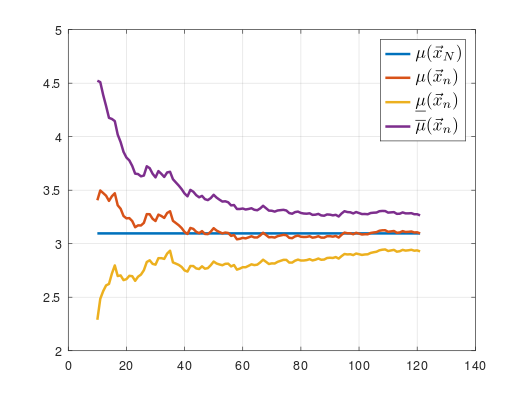
\includegraphics[scale=0.65]{./img/mu.png}
	\caption{График оценки $\mu$}
	\label{image:graph1}
\end{figure}

На рисунке \ref{image:graph2} изображены точечная оценка дисперсии $S^2(\vec{x}_n)$ и границы $\underline{\sigma^2}(\vec{x}_n)$, $\overline{\sigma^2}(\vec{x}_n)$ $\gamma$ -- доверительного интервала. Пунктирные линии демонстрируют изменение интервала при увеличении объёма данных, а горизонтальная линия — оценку $S^2(\vec{x}_N)$ для всей выборки.  

\begin{figure}[h]
	\centering
	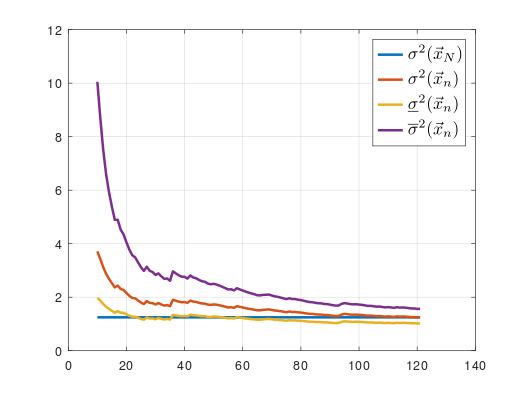
\includegraphics[scale=0.65]{./img/sigma2.png}
	\caption{График оценки $\sigma^2$}
	\label{image:graph2}
\end{figure}
